\documentclass[fleqn]{article}
\oddsidemargin 0.0in
\textwidth 6.0in
\thispagestyle{empty}
\usepackage{import}
\usepackage{amsmath}
\usepackage{graphicx}
\usepackage{flexisym}
\usepackage{calligra}
\usepackage{amssymb}
\usepackage{bigints} 
\usepackage[english]{babel}
\usepackage[utf8x]{inputenc}
\usepackage{float}
\usepackage[colorinlistoftodos]{todonotes}


\DeclareMathAlphabet{\mathcalligra}{T1}{calligra}{m}{n}
\DeclareFontShape{T1}{calligra}{m}{n}{<->s*[2.2]callig15}{}
\newcommand{\scriptr}{\mathcalligra{r}\,}
\newcommand{\boldscriptr}{\pmb{\mathcalligra{r}}\,}

\definecolor{hwColor}{HTML}{442020}

\begin{document}

  \begin{titlepage}

    \newcommand{\HRule}{\rule{\linewidth}{0.5mm}}

    \center

    \begin{center}
      
\includegraphics[height=11cm, width=11cm]{asu.png}
    \end{center}

    \vline

    \textsc{\LARGE Statistical/Thermal Physics}\\[1.5cm]

    \HRule \\[0.5cm]
    { \huge \bfseries Homework 3}\\[0.4cm] 
    \HRule \\[1.0cm]

    \textbf{Behnam Amiri}

    \bigbreak

    \textbf{Prof: Michael Treacy}

    \bigbreak

    \textbf{{\large \today}\\[2cm]}

    \vfill

  \end{titlepage}

  \begin{enumerate}
    \item \textbf{1.46} Measured heat capacities of solids and liquids are almost always at constant  pressure,
    not constant volume. To see why, estimate the pressure needed to keep $V$ fixed as $T$ increases, as follows

    \begin{enumerate}
      \item First imagine slightly increasing the temperature of a material...

        \textcolor{hwColor}{
          \\
          $\beta$ is the thermal expansion coefficient which is 
          $$
            \beta \equiv \dfrac{1}{V} \dfrac{dV}{dT}
          $$
          Fromm ideal gas law we have:
          \\
          \\
          $
            \dfrac{dV_1}{dT}=\bigg( \dfrac{dV}{dT} \bigg)_P
            \Longrightarrow dV_1=dT \bigg( \dfrac{dV}{dT} \bigg)_P
            \\
            \\
            \\
            \therefore ~~~ \boxed{
              dV_1=\beta V dT
            } ~~~~ \checkmark
          $
          \\
          \\
        }

      \item Now imagine slightly compressing the material, holding its temperature fixed...

        \textcolor{hwColor}{
          \\
          $
            \bigg( \dfrac{dV}{dP} \bigg)_T=\dfrac{dV_2}{dP}
            \Longrightarrow dV_2=dP \bigg( \dfrac{dV}{dP} \bigg)_T
            \\
            \\
            \\
            \text{Isothermal compressibility as defined as }
            \\
            \\
            \kappa_T=-\dfrac{1}{V} \bigg( \dfrac{\partial V}{\partial P} \bigg)_T
            \\
            \\
            \\
            \therefore ~~~ \boxed{
              dV_2=-V \kappa_T ~ dP
            } ~~~~ \checkmark
            \\
            \\
          $
        }

      \item Finally imagine that you compress the material just enough in part (b) to offset...

        \textcolor{hwColor}{
          \\
          $
            \text{Since the net change in volume is zero we have}
            \\
            \\
            dV_1+dV_2=0
            \\
            \\
            \begin{cases}
              dV_1=V \beta ~ dT 
              \\
              \\
              dV_2=-\kappa_T V ~ dP 
            \end{cases}
            \Longrightarrow V \beta ~ dT-\kappa_T V ~ dP=0 
            \Longrightarrow \bigg( \dfrac{\partial P}{\partial T}\bigg)_V=\dfrac{\beta}{\kappa_T}
            \\
            \\
            \\
            \Longrightarrow \boxed{\beta=\dfrac{1}{V} \bigg( \dfrac{\partial V}{\partial T} \bigg)_P}
            \\
            \\
            \\
            \text{Plugging in $\kappa_T$ and $\beta$ in $\bigg( \dfrac{\partial P}{\partial T} \bigg)=\dfrac{\beta}{\kappa_T}$ gives}
            \\
            \\
            \\
            \bigg( \dfrac{\partial P}{\partial T} \bigg)
            =-\dfrac{
              \dfrac{1}{V} \bigg( \dfrac{\partial V}{\partial T} \bigg)_P
            }{
              \dfrac{1}{V} \bigg( \dfrac{\partial V}{\partial P} \bigg)_T
            }
            \\
            \\
            \\
            \therefore ~~~ \boxed{
              \bigg( \dfrac{\partial P}{\partial T} \bigg)=-\dfrac{
                \bigg( \dfrac{\partial V}{\partial T} \bigg)_P
              }{
                \bigg( \dfrac{\partial V}{\partial P} \bigg)_T
              }
            } ~~~~ \checkmark
            \\
            \\
          $
        }

      \item Compute $\beta, \kappa_T,$ and $\bigg( \dfrac{\partial P}{\partial T} \bigg)_V$ for an ideal gas...

        \textcolor{hwColor}{
          \\
          $
            \begin{cases}
              \beta=\dfrac{1}{V} \bigg( \dfrac{\partial V}{\partial T} \bigg)_P
              =\dfrac{1}{V} \bigg( \dfrac{\partial N k T/P}{\partial T} \bigg)_P
              =\dfrac{1}{V} \dfrac{N k}{P}
              =\dfrac{1}{T}
              \\
              \\
              \kappa_T=-\dfrac{1}{V} \bigg( \dfrac{\partial V}{\partial P} \bigg)_T
              =-\dfrac{1}{V} \bigg( \dfrac{\partial NkT/P}{\partial P} \bigg)_T
              =-\dfrac{1}{V} \bigg( -\dfrac{NkT}{P^2} \bigg)=\dfrac{1}{P}
            \end{cases}
            \\
            \\
            \\
            \bigg( \dfrac{\partial P}{\partial T} \bigg)_V=\dfrac{\partial}{\partial T} \bigg( \dfrac{NkT}{V} \bigg)=\dfrac{Nk}{V}=\dfrac{P}{T}
            \\
            \\
            \\
            \therefore ~~~ \boxed{
              \bigg( \dfrac{\partial P}{\partial T} \bigg)_V=\dfrac{\beta}{\kappa_T}
            } ~~~~ \checkmark
            \\
            \\
          $
        }

      \item For water at $25^{\circ}, ~ \beta=2.57 \times 10^{-4} ~ K^{-1}$ and $\kappa_T=4.52 \times 10^{-10} ~ Pa^{-1}$...

        \textcolor{hwColor}{
          \\
          $
            dP=\dfrac{\beta}{\kappa_T} dT
            \\
            \\
            \\
            \text{Change in temperature of water}
            \\
            \\
            \\
            dT=\bigg( 30+273\bigg)-\bigg( 20+273\bigg)=10 ~ K
            \\
            \\
            \\
            dP=\dfrac{
              \bigg( 2.57 \times 10^{-4} ~ K^{-1} \bigg) \times \bigg( 10 ~ K\bigg)
            }{
              \bigg( 4.52 \times 10^{-10} ~ Pa^{-1} \bigg)
            }=5.69 \times 10^6 ~ Pa ~~~~ \text{The pressure for preventing the expansion of water}
            \\
            \\
            \\
            \\
            dP=\dfrac{
              \bigg( 1.81 \times 10^{-4} ~ K^{-1} \bigg) \times \bigg( 10 ~ K\bigg)
            }{
              \bigg( 4.04 \times 10^{-11} ~ Pa^{-1} \bigg)
            }
            =4.48 \times 10^7 ~ Pa ~~~~ \text{The pressure for preventing the expansion of mercury}
            \\
            \\
            \\
          $
          Based on the calculated results, It's a better choice to measure $C_P$ which is at constant pressure.
          \\
        }

    \end{enumerate}
    
    \item \textbf{1.47} Your $200 ~ g$ cup of tea is boiling-hot. About how much ice should you add to bring 
    it down to a comfortable sipping temperature of $65^{\circ} ~ C$? (Assume that the ice is initially 
    at $-15^{\circ} ~ C$. The specific heat capacity of ice is $0.5 ~ cal/g.^{\circ}C.$) 

        \textcolor{hwColor}{
          \\
          $
            Q=mc \Delta T=\bigg( 0.2 ~ kg \bigg) \bigg( 1 ~ cal/g.^{\circ}C. \bigg) \bigg( 100^{\circ}-65^{\circ} \bigg)
            \Longrightarrow Q=7000 ~ cal
            \\
            \\
            \\
            \text{For tea} ~~ Q=m \bigg( 0.5 ~ cal/g.^{\circ}C. \bigg) \bigg( 15^{\circ} \bigg)
            +m \bigg( 80 ~ cal/g \bigg)
            +m\bigg( 1 ~ cal/g.^{\circ}C. \bigg) \bigg( 65^{\circ} \bigg)
            \\
            \\
            \\
            \therefore ~~~ \boxed{
              m=46 ~ grams
            } ~~~~ \checkmark
            \\
            \\
          $
        }

    \item \textbf{1.54} A $60-kg$ hiker wishes to climb to the summit of Mt.Ogden an ascent of $5000$ vertical
    feet (1500 m).
    \begin{enumerate}
      \item Assuming that she is $25\%$ efficient at converting chemical energy...

        \textcolor{hwColor}{
          \\
          The potential energy due to gravity is $\Delta U_g=mg \Delta h$.
          \\
          \\
          $
            \Delta U_g=mg \Delta h=\bigg( 60 ~ kg \bigg)  \bigg( 9.8 ~ m/s^2\bigg) \bigg( 1500 ~ m \bigg)=882000 ~ J=211 ~ kilocalories
            \\
            \\
            \\ 
          $
          This hiker needs $882000 ~ J$ to get to the summit and knowing that she converts $25\%$ from chemical food 
          into mechanical energy, then for a $100\%$ she needs to receive, 
          $
            \dfrac{100\%}{25\%}=4
            \\
            \\
            \Longrightarrow 4 \times 882000=3528000 ~ J \approx 844 ~ kilocalories
            \\
            \\
          $
          Considering that standard serving is $100 ~ kilocalories$, then she roughly needs $8.5$ bowls of corn flakes.
          \\
          \\
          $
            \dfrac{844 ~ kilocalories}{100 ~ kilocalorie} \approx 8.5
          $
          \\
          \\
        }

      \pagebreak

      \item As the hiker climbs the mountain, three-quarters of the energy from...

        \textcolor{hwColor}{
          \\
          $
            \text{The total energy is } 3528000 ~ J, \text{ and three-quarters of it is } \bigg( 3528000 ~ J \bigg) \bigg( \dfrac{3}{4} \bigg)=2646000 ~ J
            \\
            \\
            Q=mc \Delta T \Longrightarrow \Delta T=\dfrac{Q}{mc}=\dfrac{2646000 ~ J}{\bigg( 60 ~ kg \bigg) \bigg( 4186 ~ J \bigg)}
            \\
            \\
            \therefore ~~~ \boxed{
              \Delta T \approx 10.53^{\circ}C
            } ~~~~ \checkmark
            \\
            \\
          $
        }

      \item In fact, the extra energy does not warm the hiker's body significantly; instead, it goes (mostly)...

        \textcolor{hwColor}{
          \\
          $
            l=\dfrac{Q}{m} \Longrightarrow m=\dfrac{2646 ~ kJ}{580 ~ kcal/kg}=\dfrac{632.5 ~ kcal}{580 ~ kcal/kg}=1.090 ~ kg
            \\
            \\
            \\
            V=\dfrac{m}{\rho}=\dfrac{1.090 ~ kg}{997 kg/m^3}=0.001 ~ m^3
            \\
            \\
            \\
            \therefore ~~~ \boxed{
              V \approx 1 ~ liter
            } ~~~~ \checkmark
            \\
            \\
          $
        }

    \end{enumerate}

    \pagebreak

    \item \textbf{2.1} Suppose you flip four fair coins.
    \begin{enumerate}
      \item Make a list of all the possible outcomes, as Table 2.1.

        \textcolor{hwColor}{
          \\
          From page 51 of the textbook we have $\Omega(N, n)=\dfrac{N!}{n! \bigg( N-n \bigg)!}$
        }

        \begin{center}
          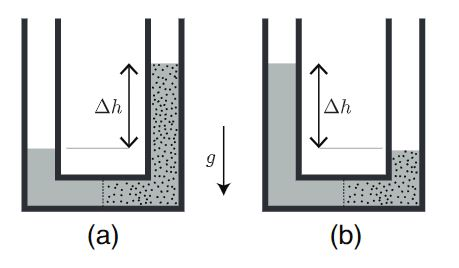
\includegraphics[height=14cm, width=11cm]{1.JPG}
        \end{center}

      \pagebreak

      \item Make a list of all different "macrostates" and their probabilities.

        \begin{center}
          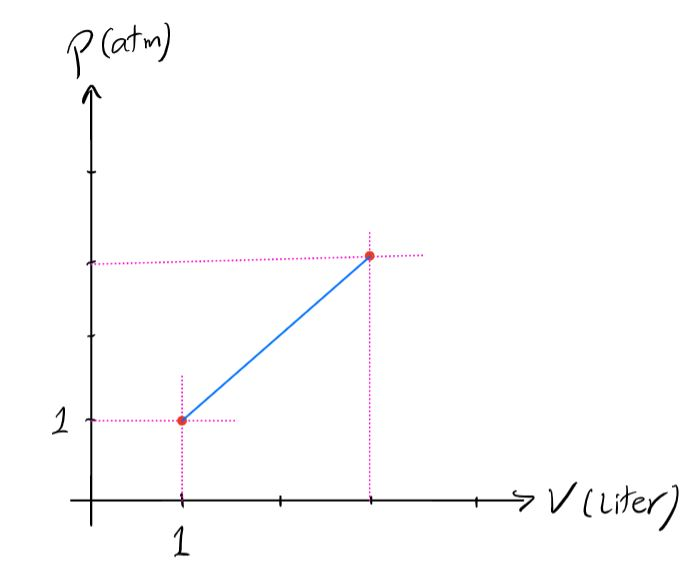
\includegraphics[height=14cm, width=11cm]{2.JPG}
        \end{center}
      
      \pagebreak

      \item Compute the multiplicity of each macrostate usuing the combinatorial formula 2.6, and check 
      that these results agree with what you got by bruteforce counting.

        \begin{center}
          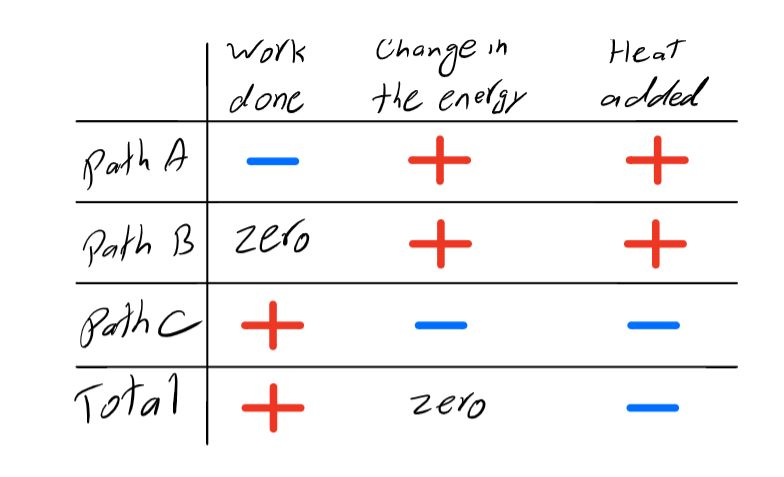
\includegraphics[height=14cm, width=11cm]{3.JPG}
        \end{center}

    \end{enumerate}

    \pagebreak

    \item \textbf{2.3} Suppose you flip 50 fair coins.
    \begin{enumerate}
      \item How many possible outcomes (microstates) are there?

        \textcolor{hwColor}{
          \\
          $
            \text{Total number of possible outcomes (heads or tails) }
            \\
            \\
            \Omega(\text{all})=2^{50} ~~~~ \checkmark
            \\
            \\
          $
        }

      \item How many ways are there of getting exacty 25 heads and 25 tails?

        \textcolor{hwColor}{
          \\
          $
            \Omega(25 ~ \text{Heads})=\dfrac{50!}{\bigg( 25! \bigg) \bigg( 25! \bigg)}
            \\
            \\
            \therefore ~~~ \boxed{
              \Omega(25 ~ \text{Heads})=1.26 \times 10^{14}
            }
            \\
            \\
          $
        }

      \item What is the probability of getting exactly 25 heads and 25 tails?

        \textcolor{hwColor}{
          \\
          $
            P(25 ~ \text{Heads})=\dfrac{\Omega(25 ~ \text{Heads})}{\Omega(\text{all})}
            =\dfrac{
              \dfrac{50!}{\bigg( 25! \bigg) \bigg( 25! \bigg)}
            }{
              2^{50}
            }
            \\
            \\
            \therefore ~~~ \boxed{
              P(25 ~ \text{Heads})=0.112
            } ~~~~ \checkmark
            \\
            \\
          $
        }

      \item What is the probability of getting exactly 30 heads and 20 tails?
      
        \textcolor{hwColor}{
          \\
          $
            P(30 ~ \text{Heads})=\dfrac{\Omega(30 ~ \text{Heads})}{\Omega(\text{all})}
            =\dfrac{
              \dfrac{50!}{\bigg( 30! \bigg) \bigg( 20! \bigg)}
            }{
              2^{50}
            }
            \\
            \\
            \therefore ~~~ \boxed{
              P(30 ~ \text{Heads})=0.041
            } ~~~~ \checkmark
            \\
            \\
          $
        }

      \item What is the probability of getting exactly 40 heads and 10 tails?

        \textcolor{hwColor}{
          \\
          $
            P(40 ~ \text{Heads})=\dfrac{\Omega(40 ~ \text{Heads})}{\Omega(\text{all})}
            =\dfrac{
              \dfrac{50!}{\bigg( 40! \bigg) \bigg( 10! \bigg)}
            }{
              2^{50}
            }
            \\
            \\
            \therefore ~~~ \boxed{
              P(30 ~ \text{Heads})=9.12 \times 10^{-6}
            } ~~~~ \checkmark
            \\
            \\
          $
        }

      \item What is the probability of getting 50 heads and no tails?

        \textcolor{hwColor}{
          \\
            $
            P(50 ~ \text{Heads})=\dfrac{\Omega(50 ~ \text{Heads})}{\Omega(\text{all})}
            =\dfrac{
              \dfrac{50!}{\bigg( 50! \bigg) \bigg( 0! \bigg)}
            }{
              2^{50}
            }
            \\
            \\
            \therefore ~~~ \boxed{
              P(30 ~ \text{Heads})=8.88 \times 10^{-16}
            } ~~~~ \checkmark
            \\
            \\
          $
        }

      \item Plot a graph of the probability of getting n heads, as a function of n.

      \begin{center}
        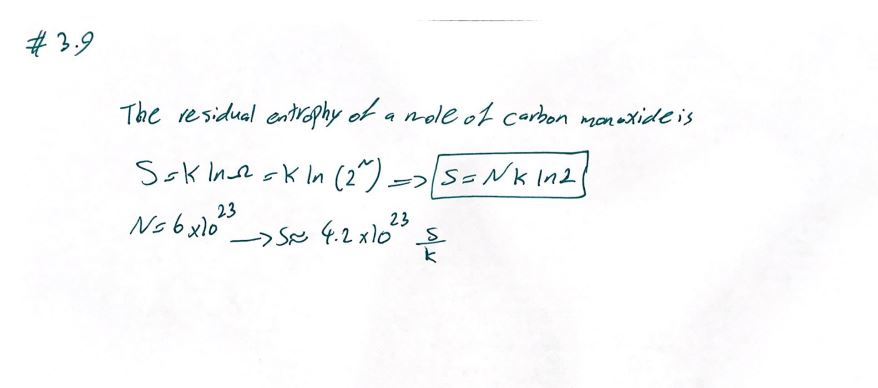
\includegraphics[height=12cm, width=15cm]{4.JPG}
      \end{center}

    \end{enumerate}

    \pagebreak

    \item \textbf{2.10} Use a computer to produce a table and graph, like those in this section, for the case
    where one Einstein solid contains 200 oscillators, the other contains 100 oscillator, and there are 
    100 units of energy in total. What is the most probable macrostate, and what is its probability? What
    is the least probable macrostate, and what is its probability?

        % \textcolor{hwColor}{
        %   \\
        % }

  \end{enumerate}

\end{document}
